\documentclass{article}
\usepackage[utf8]{inputenc}
\usepackage{fancyhdr}
\usepackage{graphicx}
\usepackage{hyperref}

% ---- Commands ------- %
\newcommand{\documentNumber}[1]{
    \LARGE  \textbf{ PUSP2142{#1} } \\
    \medskip
}
\newcommand{\documentVersion}[1]{
    v.{#1} \\
    \medskip
}
\newcommand{\documentTitle}[1]{
    \centerline{\rule{13cm}{0.4pt}}
    \bigskip \bigskip
    \LARGE {#1} \\
    \bigskip \bigskip
    \centerline{\rule{13cm}{0.4pt}}
}
\newcommand{\documentGroup}[1]{
    \bigskip \bigskip
    \LARGE Group {#1} \\
    \bigskip
}
\newcommand{\documentResponsible}[1]{
    \LARGE Responsible: {#1} \\
    \medskip
}
\newcommand{\documentAuthors}[1]{
    \LARGE Authors: {#1} \\
    \medskip    
}
\newcommand{\documentDate}[1]{
    \date {#1} 
}


% --- Header & Footer ---- %
\pagestyle{fancy}
\lhead{\leftmark}
\rhead{}
\rfoot{\thepage}
\cfoot{}
\lfoot{}


% ------------------------------------------------ #


\title {
    \documentNumber {01}    % Must be 2 digits
    \documentVersion {0.1}
    \documentTitle {Software development plan - SDP}
    \documentGroup {2}
    \documentResponsible {(PG) Projet-management Group}
    \documentAuthors {(PG) Projet-management Group}
    \documentDate {\today}
}

\begin{document}

\maketitle
\thispagestyle{empty}

\newpage

\tableofcontents

\newpage

\section{Introduction}
    Hej detta e en introduktion
    
    ORDLISTA?
    
    \textbf{NOTE}
    I samband med projektplanen är det också viktigt att tänka på att det i slutet
    av projektet skall skrivas en slutrapport. Detta betyder att man redan vid skri-
    vandet av planen bör överväga hur slutrapporten skall se ut så att man enkelt
    kan stämma av med projektplanen.

\section{Referenced documents}
    \begin{itemize}
        \item \href{https://google.github.io/styleguide/javaguide.html}{Google Java Style Guide}
        \item PUSS214201
    \end{itemize}
    
    


\section{Terminology}
    \renewcommand{\arraystretch}{1.7}  % Vertical padding for tables
    
    \begin{table}[h]
        \centering
        \begin{tabular}{| p{1cm} | p{10cm} |}
            \hline 
                CML & Configuration Management List, consists of all configuration units \\
            \hline            
                ECG & Error Control Group, consists of PG and SG \\
            \hline
        \end{tabular}
    \end{table}
    

\section{Development model} %Assar och Victor
    The development model that is used in this project is the waterfall model. This
    means that the project is divided into four seperate phases where each phase depends
    on the previous one in a sequential manner. It is thus required that a phase is
    completed before the next one begins.
    \\ \\
    In every phase, there are several documents that must be produced and a phase
    is considered completed only once all documents required in the phase has reached baseline.
    To reach baseline, all documents of the phase must first pass an informal review, 
    followed by a formal review.
    
\section{Staff organisation} %Assar

    \subsection{Client}
    
    \subsection{Head of section}
    
    \subsection{Experts}
    
    \subsection{Examiner}
    
    \subsection{Project managment group}
        \subsection{Documents and tasks}
            The project management group is resposible for coordinating the group effort and ensuring that the end product meets the specification. 
            
            
            
            The project management group will author the following documents
            \begin{itemize}
                \item Software development plan
                \item System specification document
                \item Project final report
            \end{itemize}
    
    \subsection{Software architecture group}
            
    \subsection{Development group}
    
    \subsection{Quality control group}

\newpage

\section{Schedule}
    \subsection{Estimated phase schedule}
        \begin{table}[h]
            \centering
            \begin{tabular}{|c|c|c|c|c|}
                \hline
                            & Phase 1 & Phase 2 & Phase 3 & Phase 4 \\
                 \hline
                 Start      & Week 3  & Week 7  & Week 8  & Week 10  \\
                 \hline
                 Stop       & Week 6  & Week 7  & Week 9  & Week 12  \\
                 \hline
            \end{tabular}
            \caption{Estimated start and end weeks for the phases}
        \end{table}
    
    
    \section{Estimated work load}
        
    \subsection{Reviews}
        Reviews will be carried out during the last week of any phase, we have also chosen to perform informal reviews with a one day margin for eventual corrections. Informal and formal reviews are scheduled for Wednesdays and Fridays respectively. Should the formal review reveal any discrepencies between docuemnts, or fail for any other reason, a second review will be held on the following monday.
    
    \subsection{}

\section{Standards \& tools}    % Victor
    In order to make the development process as easy and straight forward as possible,
    the project group has agreed on several standards and tools to use. 
    \\ \\
    The standards should be followed by every member and consists of the following:
    \begin{itemize}
        \item The soure code should follow the
        \href{https://google.github.io/styleguide/javaguide.html}{Google Java Style Guide}.
        \item All comments, commits and pull-requests should be in english.
    \end{itemize}
    
    \subsection{Discord}
    Discord is used as the many communcation tool in the group. A server has been setup and is
    used for both messaging, working together and having project meetings.
    The server consistst of several voice channels and several text channels, each
    with its specific purpose, eg "Meetings" or "Developer Group".
    
    \subsection{Github \& Git}
    Git is used for collaboration between decouments and the project library (see 8.1)
    and is hosted on Github. Git provides abilities that  makes certain action very
    easy, such as pulling and pushing updates to the working repository and creating pull-requests for merging.
    
    \subsection{Eclipse}
        Eclipse is the primary IDE that is used due to its familarity in
        the group and its huge span of different properties such as plugins.
    
        \subsubsection{Egit}
            Egit is a plugin for Eclipse that provides the tools needed for a git workflow 
            in Eclipse IDE.
            
        \subsubsection{TeXlipse}
            TeXlipse is a plugin that provides the tools needed to compile and preview
            latex files directly in Eclipse IDE.
    

\section{Configuration managment}   % Victor
    Git and Github are the tools that are used to handle configuration management.

    \subsection{Project library}
        The project library consists of two seperate libraries: Document libray and Work library.
    
        \subsubsection{Document library}
            The document library consists of all configuration units that have reached baseline.
            The purpose of this library is that the customer or a reviewer at any point should
            be able to access these documents.
            This means that this library is initially empty, and documents are added as the project proceeds.
            \\ \\
            \textbf{ALTERNATIVT referera till CML?}
            This library consists of:
            \begin{itemize}
                \item Software Development Plan (SDP)
                \item Software Requirements Specification (SRS)
                \item Software Verification and Validation Specification (SVVS)
                \item Software Verification and Validation Instruction (SVVI)
                \item Software Top Level Design Document (STLDD)
                \item Software Detailed Design Document (SDDD)
                \item Software Verification and Validation Report (SVVR)
                \item System Specification Document (SSD)
            \end{itemize}
            
        \subsubsection{Work library}
            The work library contains everything all files that are required during the project.
            The library is divided into three different branches where each branch has a unique purpose.
            
            \begin{itemize}
                \item \textbf{development} \\
                This branch is where the all development is made and is used as a placement for all files related
                to the project, regardless of the documents status.
                Every member in the group has free write access to this branch.
                
                \item \textbf{review} \\
                Once the documents in the development branch are ready for a formal review,  they are moved
                into the \textbf{review} branch. This requires a pull-request to be made, which must be
                reviewed and accepted by a reviewer before it is merged into the branch.
                
                \item \textbf{master} \\
                Once the documents pass the formal reviews, they are merged into \textbf{master} branch,
                which consists of only files that have reached baseline.
                Once new documents are added to this branch, they are also placed in the \textbf{document library}.
                Note that not all files are copied to the document library, but only the documents specified above.
                
            \end{itemize}
            
            \begin{figure}[h]
                \centering
                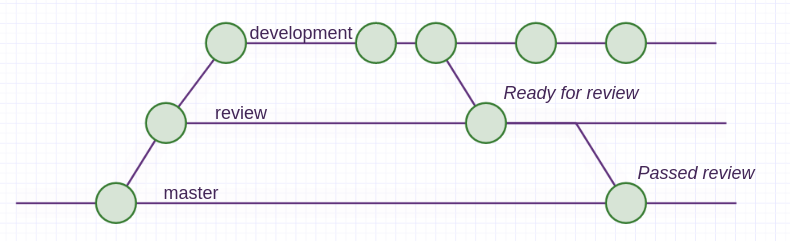
\includegraphics[scale=0.45]{images/workflow.png}
                \caption{Workflow of the \textbf{Work Library}}
                \label{bigdog}
            \end{figure}
        
    \subsection{Bug management}
    
    \subsection{Patch management}
        Once a configuration unit has reached baseline there are several steps
        that must be taken in order to make changes to it.
        These steps consists of the following:
        \begin{enumerate}
            \item Creating a problem report that states what the
                    problem is with the unit, in its current state.
            \item The problem report is handled to the ECG who creates a 
                    status report. ECG must then decide if the problem was
                    in fact a real problem or not.
            \item If ECG decides that it was indeed a problem, then they
                    give a proposal for a solution to the problem to
                    the 
                
        \end{enumerate}
        

    \section{Version update}

\section{Rules and guidelines} %Assar
    
\section{Follow up and quality evaluation}

Det ska finnas en del i projektplanen som beskriver hur uppföljning, t ex av
tidplanen, sker under projektet, samt vad som händer om arbetet inte verkar
gå enligt plan. Det ska också finnas en beskrivning av de rutiner som finns för
kvalitetsutvärdering under projektet.

    

\section{Risk anlysis}

I projektplanen ska även resultatet av en riskanalys för projektet presenteras.
Ange hur riskanalys utförts i projektet, samt de viktigaste riskerna som identi-
fierats. rapportera åtminstone följande för varje rapporteras risk: skattad san-
nolikhet (t ex, låg, medel, hög), skattad effekt (t ex, låg, medel, hög), möjliga
indikatorer på att risken förvekligas, samt exempel på lösningar om risken för-
verkligas.


\end{document}
